\documentclass[11pt,a4paper]{article}

\usepackage[left=2cm, right=2cm, top=2cm, bottom=2cm]{geometry}
\usepackage{graphicx}
\usepackage{mathtools}
\usepackage{amssymb}
\usepackage{hyperref}
\usepackage{siunitx}
\usepackage[version=4]{mhchem}
\usepackage{tabularray}
\usepackage[square,sort,comma,numbers]{natbib}

\title{xxx: Supporting information}
\author{Pierre Beaujean}
\begin{document}
\maketitle


\renewcommand{\thetable}{S\arabic{table}}
\renewcommand{\thefigure}{S\arabic{figure}}

\begin{figure}[!h]
	\centering
	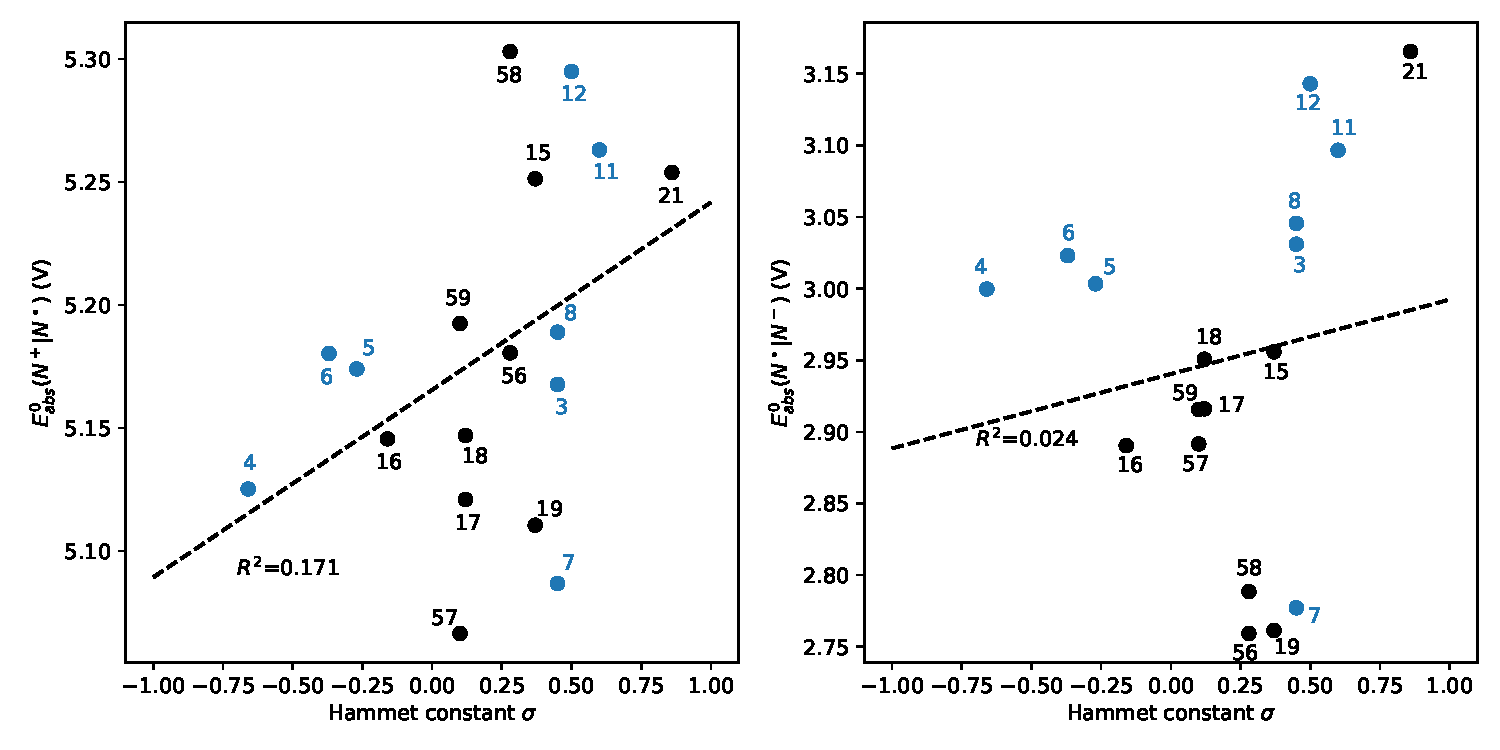
\includegraphics [width=\linewidth]{FigureS1}
	\caption{Evolution of the Born solvatation energy, $\Delta G^\star_{Born}$ (computed with Eq.~(4) of the main text) with the dielectric constant of the solvent (left) for different spherical cavities ($a$) and of the Debye-Huckel correction, $\Delta G^\star_{DH}$  (computed with Eq.~(5) of the main text) with the concentration in electrolyte, $[X]$ (right) in water and acetontrile.}
\end{figure}

\begin{figure}[!h]
\centering
\includegraphics [width=.5\linewidth]{FigureS2}
\caption{Impact of the concentration of electrolyte on the formal oxidation potential (computed with Eq.~(9) of the main  text), $E^f_{abs}$, considering a fictitious case where $E^0_{abs} = \SI{0}{\volt}$.}
\end{figure}

\begin{figure}[!h]
\centering
\includegraphics [width=.7\linewidth]{FigureS3}
\caption{Evolution of the pairing energy, $\Delta G^\star_{pair}$ (computed with Eq.~(11) of the main text) between two ions, with the ratio between the radii of the two ions ($\chi$) and for increasing dipole cavity shapes ($s_2$). Their charge is set to 1 and -1, and two possible scaling for  the close contact distance is used ($s_1$, left and right). The equilibrium constant, $K_{pair} = e^{-\frac{\Delta G^\star_{pair}}{RT}}$, is reported. }
\end{figure}


\begin{figure}[!h]
	\centering
	\includegraphics [width=.7\linewidth]{FigureS4}
	\caption{Comparison between the absolute oxidation (ltop) and reduction (bottom) potentials obtained by Hodgson \emph{et al.} (at the G3(MP2)-RAD:MP2/6-311+G(3df,2p) level, using solvation energy computed at the B3LYP/6-31G(d) level in water [CPCM]) \cite{hodgsonOneElectronOxidationReduction2007}, and in this work (at the $\omega$B97X-D/6-311+G(d) level in water [SMD]). The DH correction has \textbf{not} been applied. The large differences (e.g., for the oxidation of APOs) are due to change in geometries after re-optimization.}
\end{figure}

\clearpage
\begin{longtblr}[caption={Radii ($a$, in \si{\angstrom}) for all oxidized states of compounds \textbf{1}-\textbf{61} and corresponding absolute redox potentials ($E^0_{abs}$, in \si{\volt}), as computed at the $\omega$B97X-D/6-311+G(d) level in water (SMD), with $[\ce{X}]=\SI{0}{\mole\per\liter}$.}]{colspec={>{\bfseries}lX[c]X[c]X[c]X[c]X[c]},width = 0.85\linewidth, rowhead=1}
	\hline
	& $a_{\ce{N+}}$ & $a_{\ce{N^.}}$ & $a_{\ce{N-}}$ & $E^0_{abs}(\ce{N+}|\ce{N^.})$ & $E^0_{abs}(\ce{N^.}|\ce{N-})$\\
	\hline
	1 & 3.40 & 3.38 & 3.39 & 5.00 & 2.88\\
	2 & 3.33 & 3.30 & 3.34 & 5.09 & 2.97\\
	3 & 3.92 & 3.91 & 3.90 & 5.17 & 3.03\\
	4 & 3.36 & 3.35 & 3.35 & 5.13 & 3.00\\
	5 & 3.91 & 3.91 & 3.91 & 5.18 & 3.00\\
	6 & 3.31 & 3.30 & 3.34 & 5.18 & 3.02\\
	7 & 4.27 & 4.47 & 4.46 & 5.09 & 2.77\\
	8 & 4.06 & 4.05 & 4.06 & 5.19 & 3.04\\
	9 & 4.05 & 4.04 & 4.05 & 5.29 & 3.13\\
	10 & 4.16 & 4.16 & 4.16 & 5.32 & 3.14\\
	11 & 3.37 & 3.36 & 3.36 & 5.29 & 3.10\\
	12 & 3.33 & 3.31 & 3.34 & 5.30 & 3.14\\
	13 & 3.28 & 3.30 & 3.34 & 5.14 & 2.99\\
	14 & 3.27 & 3.27 & 3.24 & 5.08 & 2.84\\
	15 & 3.57 & 3.82 & 3.74 & 5.26 & 2.95\\
	16 & 3.27 & 3.26 & 3.24 & 5.15 & 2.89\\
	17 & 3.47 & 3.48 & 3.85 & 5.13 & 2.91\\
	18 & 3.25 & 3.25 & 3.24 & 5.15 & 2.95\\
	19 & 4.20 & 4.19 & 4.33 & 5.11 & 2.76\\
	20 & 3.81 & 3.81 & 3.81 & 5.33 & 3.03\\
	21 & 3.27 & 3.24 & 3.23 & 5.28 & 3.17\\
	22 & 3.24 & 3.23 & 3.18 & 5.35 & 3.10\\
	23 & 3.60 & 3.60 & 3.62 & 5.27 & 2.96\\
	24 & 4.58 & 4.58 & 4.62 & 5.29 & 3.07\\
	25 & 4.05 & 4.02 & 4.01 & 5.23 & 2.96\\
	26 & 4.65 & 4.66 & 4.69 & 5.23 & 2.98\\
	27 & 3.94 & 3.94 & 3.98 & 5.24 & 2.99\\
	28 & 5.01 & 5.00 & 5.07 & 5.24 & 2.79\\
	29 & 4.30 & 4.29 & 4.24 & 5.28 & 3.08\\
	30 & 4.32 & 4.32 & 4.35 & 5.36 & 3.12\\
	31 & 4.61 & 4.60 & 4.62 & 5.32 & 3.12\\
	32 & 4.57 & 4.57 & 4.58 & 5.34 & 3.11\\
	33 & 4.63 & 4.64 & 4.65 & 5.34 & 3.04\\
	34 & 4.69 & 4.71 & 4.24 & 5.27 & 3.01\\
	35 & 4.05 & 4.04 & 4.07 & 5.34 & 3.06\\
	36 & 4.13 & 4.14 & 4.13 & 5.24 & 3.10\\
	37 & 4.58 & 4.62 & 4.61 & 5.26 & 3.15\\
	38 & 5.21 & 5.18 & 5.00 & 5.30 & 3.08\\
	39 & 5.10 & 5.09 & 5.11 & 5.30 & 3.15\\
	40 & 5.19 & 5.10 & 5.17 & 5.31 & 3.19\\
	41 & 5.09 & 5.05 & 5.06 & 5.29 & 3.21\\
	42 & 5.08 & 5.12 & 5.00 & 5.33 & 3.08\\
	43 & 5.47 & 5.49 & 5.68 & 5.31 & 3.15\\
	44 & 5.32 & 5.41 & 5.46 & 5.29 & 3.22\\
	45 & 5.21 & 4.90 & 4.98 & 5.31 & 3.19\\
	46 & 5.14 & 5.17 & 5.15 & 5.32 & 3.16\\
	47 & 5.22 & 5.22 & 5.55 & 5.29 & 3.13\\
	48 & 5.12 & 5.13 & 4.79 & 5.31 & 3.16\\
	49 & 4.13 & 4.14 & 4.14 & 5.14 & 3.07\\
	50 & 4.56 & 4.52 & 4.57 & 5.24 & 3.08\\
	51 & 4.52 & 4.50 & 4.49 & 5.19 & 3.06\\
	52 & 4.11 & 4.12 & 4.12 & 5.35 & 3.19\\
	53 & 4.74 & 4.71 & 4.68 & 5.36 & 3.13\\
	54 & 4.63 & 4.64 & 4.65 & 5.33 & 3.17\\
	55 & 4.67 & 4.68 & 4.67 & 5.41 & 3.23\\
	56 & 3.80 & 3.85 & 3.88 & 5.18 & 2.76\\
	57 & 3.57 & 3.54 & 3.60 & 5.07 & 2.89\\
	58 & 3.67 & 3.65 & 3.64 & 5.31 & 2.78\\
	59 & 3.63 & 3.62 & 3.65 & 5.20 & 2.91\\
	60 & 4.01 & 4.00 & 4.01 & 5.31 & 3.04\\
	61 & 3.31 & 3.30 & 3.34 & 5.20 & 3.06\\
	\hline
\end{longtblr}

\clearpage
\begin{longtblr}[caption={Absolute redox potentials ($E^0_{abs}$, in \si{\volt}) computed at the $\omega$B97X-D/6-311+G(d) level in gas phase.}]{colspec={>{\bfseries}lX[c]X[c]c>{\bfseries}lX[c]X[c]},width = 0.85\linewidth, rowhead=1}
\hline
& $E^0_{abs}(\ce{N+}|\ce{N^.})$ & $E^0_{abs}(\ce{N^.}|\ce{N-})$ &&& $E^0_{abs}(\ce{N+}|\ce{N^.})$ & $E^0_{abs}(\ce{N^.}|\ce{N-})$\\
\hline
1  & 6.69 & 0.18 &  & 32 & 7.22 & 0.57 \\ 
2 & 7.01 & 0.23 &  & 33 & 7.33 & 0.60 \\ 
3 & 7.16 & 0.41 &  & 34 & 6.98 & 0.32 \\ 
4 & 7.06 & 0.31 &  & 35 & 9.93 & 3.04 \\ 
5 & 7.09 & 0.33 &  & 36 & 7.04 & 0.52 \\ 
6 & 7.12 & 0.40 &  & 37 & 6.97 & 0.65 \\ 
7 & 6.89 & 0.41 &  & 38 & 7.12 & 0.67 \\ 
8 & 7.15 & 0.46 &  & 39 & 7.11 & 0.73 \\ 
9 & 7.28 & 0.64 &  & 40 & 6.99 & 0.75 \\ 
10 & 7.27 & 0.69 &  & 41 & 7.06 & 0.82 \\ 
11 & 10.41 & 3.54 &  & 42 & 7.07 & 0.74 \\ 
12 & 7.40 & 0.63 &  & 43 & 7.07 & 0.78 \\ 
13 & 7.08 & 0.23 &  & 44 & 7.00 & 0.75 \\ 
14 & 7.04 & 0.03 &  & 45 & 7.17 & 0.78 \\ 
15 & 7.20 & 0.29 &  & 46 & 7.17 & 0.85 \\ 
16 & 7.01 & 0.14 &  & 47 & 7.19 & 0.81 \\ 
17 & 6.95 & 0.13 &  & 48 & 7.20 & 0.88 \\ 
18 & 7.01 & 0.33 &  & 49 & 6.80 & 0.51 \\ 
19 & 6.93 & 0.36 &  & 50 & 6.91 & 0.49 \\ 
20 & 7.30 & 0.50 &  & 51 & 6.76 & 0.46 \\ 
21 & 10.82 & 6.26 &  & 52 & 7.20 & 0.82 \\ 
22 & 7.37 & 0.31 &  & 53 & 7.34 & 0.87 \\ 
23 & 7.12 & 0.28 &  & 54 & 7.32 & 0.92 \\ 
24 & 7.25 & 0.47 &  & 55 & 7.62 & 1.26 \\ 
25 & 6.93 & 0.19 &  & 56 & 6.91 & 0.22 \\ 
26 & 7.02 & 0.24 &  & 57 & 6.88 & 0.15 \\ 
27 & 7.08 & 0.29 &  & 58 & 7.22 & 0.24 \\ 
28 & 7.00 & 0.44 &  & 59 & 7.03 & 0.06 \\ 
29 & 7.06 & 0.35 &  & 60 & 7.26 & 0.45 \\ 
30 & 6.98 & 0.51 &  & 61 & 7.28 & 0.57 \\ 
31 & 7.17 & 0.55 &  &  &  &  \\ 
\hline
\end{longtblr}

\clearpage
\begin{longtblr}[caption={Radii ($a$, in \si{\angstrom}) for all oxidized states of the compounds and corresponding absolute redox potentials ($E^0_{abs}$, in \si{\volt}), as computed at the $\omega$B97X-D/6-311+G(d) level in acetontrile (SMD), with $[\ce{X}]=\SI{0}{\mole\per\liter}$.}]{colspec={>{\bfseries}lX[c]X[c]X[c]X[c]X[c]},width = 0.85\linewidth, rowhead=1}
	\hline
	& $a_{\ce{N+}}$ & $a_{\ce{N^.}}$ & $a_{\ce{N-}}$ & $E^0_{abs}(\ce{N+}|\ce{N^.})$ & $E^0_{abs}(\ce{N^.}|\ce{N-})$\\
	\hline
	2 & 3.33 & 3.30 & 3.35 & 4.99 & 2.32\\
	3 & 3.92 & 3.91 & 3.90 & 5.15 & 2.37\\
	4 & 3.36 & 3.36 & 3.35 & 5.06 & 2.34\\
	6 & 3.31 & 3.30 & 3.35 & 5.11 & 2.37\\
	12 & 3.33 & 3.31 & 3.34 & 5.57 & 2.46\\
	15 & 3.58 & 3.81 & 3.74 & 5.20 & 2.30\\
	23 & 3.61 & 3.60 & 3.62 & 5.24 & 2.33\\
	24 & 4.59 & 4.57 & 4.62 & 5.27 & 2.37\\
	25 & 4.05 & 4.03 & 4.02 & 5.19 & 2.30\\
	26 & 4.65 & 4.65 & 4.68 & 5.22 & 2.31\\
	27 & 3.95 & 3.94 & 3.98 & 5.23 & 2.32\\
	33 & 4.63 & 4.64 & 4.65 & 5.28 & 2.42\\
	36 & 4.13 & 4.12 & 4.08 & 5.19 & 2.51\\
	51 & 4.53 & 4.50 & 4.47 & 5.12 & 2.47\\
	54 & 4.61 & 4.62 & 4.63 & 5.33 & 2.58\\
	55 & 4.68 & 4.68 & 4.62 & 5.40 & 2.68\\
	58 & 3.66 & 3.65 & 3.64 & 5.24 & 2.12\\
	59 & 3.62 & 3.61 & 3.65 & 5.14 & 2.27\\
	60 & 4.01 & 3.99 & 4.02 & 5.28 & 2.36\\
	61 & 3.31 & 3.30 & 3.34 & 5.15 & 2.42\\
	\hline
\end{longtblr}

\clearpage

\begin{figure}[!h]
	\centering
	\begin{tblr}{lcc}
		\hline
		& $\sigma_p$ & $\sigma_m$ \\
		\hline
		\ce{COOH} & 0.45 &0.37 \\
		\ce{NH2} & -0.66 & -0.16 \\
		\ce{OMe} & -0.27 & 0.12 \\
		\ce{OH} & -0.37 & 0.12 \\
		\ce{NH3+} & 0.60 & 0.86 \\
		\ce{Br} & 0.23 & 0.39 \\
		$>$\ce{C=O} & 0.50 & --- \\
		\ce{C=C-CONH2} & 0.36 & 0.28 \\
		\ce{NO2} & 0.78 & 0.71 \\
		\hline
	\end{tblr}
	\includegraphics [width=\linewidth]{FigureS5}
	\caption{Correlation between absolute oxidation (left) and reduction (right) and the Hammet constant of their substituent (para, $\sigma_p$, or meta, $\sigma_m$, from Ref.~\cite{hanschSurveyHammettSubstituent1991} and reported in the table) for compounds of the P5O (black markers, correlated with $\sigma_m$) and P6O (blue markers, with correlated with $\sigma_p$) families.}
\end{figure}

\clearpage

\begin{longtblr}[caption={Distance ($r$, in \si{\angstrom}), $x$-component of the dipole moment  ($\mu_x$, in \si{\elementarycharge\bohr}) and $xx$ component of the traceless quadrupole moment  ($Q_{xx}$, in \si{\elementarycharge\bohr\squared}) for all compounds, as computed at the $\omega$B97X-D/6-311+G(d) level in gas phase for model geometries ($>$\ce{N-O^.} replaced by \ce{CH2}, see main text) }]{colspec={>{\bfseries}lX[c]X[c]X[c]}, width = 0.85\linewidth, rowhead=1}
	\hline
	& $r$ & $\mu_x$ & $Q_{xx}$\\
	\hline
	2 & 2.87 & -0.05 & -0.06\\
	3 & 2.87 & 0.29 & 3.36\\
	4 & 2.89 & 0.33 & -1.26\\
	5 & 2.87 & 0.19 & 0.99\\
	6 & 2.87 & 0.73 & -2.41\\
	7 & 2.86 & 0.35 & 3.14\\
	8 & 2.86 & 0.29 & 1.94\\
	9 & 2.86 & 0.63 & 3.10\\
	10 & 2.85 & 0.80 & -0.49\\
	12 & 2.83 & 1.28 & -1.44\\
	13 & 2.80 & 0.06 & 0.64\\
	14 & 2.20 & -0.02 & -0.03\\
	15 & 2.20 & 0.29 & 2.22\\
	16 & 2.20 & 0.42 & -2.33\\
	17 & 2.21 & -0.33 & 1.09\\
	18 & 2.21 & -0.03 & 0.10\\
	19 & 2.20 & 0.34 & 1.26\\
	20 & 2.19 & 0.77 & 0.35\\
	22 & 2.15 & 0.62 & -0.24\\
	23 & 2.19 & 0.17 & 2.74\\
	24 & 2.19 & 0.61 & 7.84\\
	25 & 2.19 & -0.27 & 2.42\\
	26 & 2.19 & 0.18 & 1.13\\
	27 & 2.19 & 0.03 & 3.80\\
	28 & 2.18 & 0.60 & 7.36\\
	29 & 2.19 & -0.01 & 4.95\\
	30 & 2.18 & -0.36 & 3.30\\
	31 & 2.18 & -0.11 & 11.49\\
	32 & 2.19 & 0.70 & 5.41\\
	33 & 2.18 & 1.14 & 6.51\\
	34 & 2.19 & -0.22 & 5.34\\
	36 & 2.81 & 0.26 & 4.61\\
	37 & 2.81 & 0.31 & 5.55\\
	38 & 2.82 & 0.50 & 9.83\\
	39 & 2.83 & 0.77 & 8.60\\
	40 & 2.81 & 0.68 & 7.29\\
	41 & 2.81 & 0.45 & 12.13\\
	42 & 2.82 & 0.96 & 5.67\\
	43 & 2.81 & -0.43 & 1.02\\
	44 & 2.81 & -0.07 & 5.29\\
	45 & 2.82 & 1.42 & 4.35\\
	46 & 2.83 & 0.25 & 10.50\\
	47 & 2.81 & -0.17 & 7.36\\
	48 & 2.82 & 1.19 & 10.49\\
	49 & 2.79 & -0.21 & 4.30\\
	50 & 2.82 & -0.15 & 4.82\\
	51 & 2.82 & -0.16 & 4.23\\
	52 & 2.81 & 1.01 & 7.74\\
	53 & 2.82 & 2.18 & 3.27\\
	54 & 2.83 & 2.37 & 2.41\\
	55 & 2.83 & 3.96 & 6.84\\
	56 & 2.22 & -0.19 & 2.94\\
	57 & 2.21 & 0.36 & -3.39\\
	58 & 2.19 & 0.28 & 2.91\\
	59 & 2.19 & -0.15 & 2.12\\
	60 & 2.19 & 0.98 & 2.98\\
	61 & 2.85 & 1.01 & -0.94\\
	\hline
\end{longtblr}


\clearpage
\begin{longtblr}[caption={Distances ($d$, in \si{\angstrom}) between \ce{N+} and \ce{A-} (left, measured as the distance between the nitrogen of \ce{N+} and the boron of \ce{A-}) and between \ce{N-} and \ce{C+} (right, measured as the distance between the nitrogen of \ce{N-} and the nitrogen of \ce{C+}) tohether with their corresponding free Gibbs energy of complexation ($\Delta G^\star_{cplx}$, in \si{\kilo\joule\per\mole}) in two different cases: in front of the methyls ($f$, near the redox center) and behind the methyls ($b$, near the substituent), as computed at the $\omega$B97X-D/6-311+G(d) level in water (SMD), with $[\ce{X}]=\SI{0}{\mole\per\liter}$.}]{colspec={>{\bfseries}lX[c]X[c]X[c]X[c]cX[c]X[c]X[c]X[c]}, width = \linewidth,rowhead=2}
\hline
&  \SetCell[c=4]{c} \ce{NA} & & & & &  \SetCell[c=4]{c} \ce{NC} &  & & \\ 
\cline{2-5} \cline{7-10}
& $d_f$ &  $\Delta{G}_{cplx,f}^\star$ &  $d_b$ &  $\Delta{G}_{cplx,b}^\star$ &&  $d_f$ &  $\Delta{G}_{cplx,f}^\star$ & $d_b$ &  $\Delta{G}_{cplx,b}^\star$\\
\hline
2 & 4.04 & 20.8 & 4.13 & 17.6 &  & 4.13 & 46.9 & 4.38 & 45.9\\
3 & 4.06 & 20.8 & 4.07 & 18.2 &  & 3.83 & 46.1 & 4.06 & 45.8\\
4 & 4.05 & 18.4 & 4.70 & 14.5 &  & 3.92 & 46.2 & 4.15 & 41.4\\
5 & 4.06 & 15.0 & 4.06 & 16.5 &  & 3.77 & 44.8 & 4.26 & 37.1\\
6 & 4.49 & 20.9 & 4.87 & 13.9 &  & 3.91 & 45.9 & 4.16 & 44.4\\
7 & 4.40 & 20.5 & 4.77 & 18.7 &  & --- & --- & 3.87 & 39.9\\
8 & 4.00 & 22.0 & 5.75 & 18.6 &  & 4.07 & 55.1 & 4.71 & 49.1\\
9 & 4.04 & 23.4 & 4.87 & 22.7 &  & 4.33 & 58.1 & 3.74 & 55.1\\
10 & 4.10 & 25.7 & 5.92 & 17.7 &  & 4.54 & 47.3 & 4.09 & 47.5\\
11 & --- & --- & 4.87 & 6.7 &  & 3.81 & 44.1 & 4.07 & 40.0\\
12 & --- & --- & 4.01 & 12.0 &  & 3.83 & 41.7 & 4.43 & 34.9\\
13 & 3.84 & 21.6 & 5.27 & 20.6 &  & 4.26 & 22.0 & 6.50 & 24.0\\
14 & 4.25 & 19.0 & 5.40 & 19.4 &  & 4.10 & 24.4 & 7.08 & 25.2\\
15 & 4.07 & 26.6 & --- & --- &  & 3.89 & 21.1 & 7.13 & 34.8\\
16 & 4.07 & 25.1 & 4.20 & 24.3 &  & 4.88 & 37.7 & 6.73 & 26.0\\
17 & 4.06 & 16.9 & 5.67 & 22.7 &  & 4.66 & 25.6 & --- & ---\\
18 & 4.07 & 21.3 & --- & --- &  & 4.87 & 32.1 & 7.52 & 34.7\\
19 & 4.45 & 35.9 & --- & --- &  & 3.70 & 28.5 & 5.83 & 24.3\\
20 & 4.18 & 54.5 & 4.63 & 57.4 &  & 3.90 & 32.9 & --- & ---\\
21 & 4.38 & 24.8 & 5.14 & 13.9 &  & 4.12 & 21.2 & --- & ---\\
22 & 4.00 & 20.0 & 5.51 & 20.4 &  & 3.99 & 22.8 & 6.80 & 25.9\\
23 & 4.21 & 18.7 & 5.01 & 20.5 &  & 4.85 & 24.7 & 6.27 & 15.5\\
24 & 4.19 & 20.3 & 5.51 & 18.9 &  & 4.20 & 25.5 & 6.62 & 13.8\\
25 & 4.12 & 19.5 & 5.55 & 19.0 &  & 4.96 & 26.2 & 6.51 & 15.1\\
26 & 4.11 & 24.9 & 5.57 & 22.7 &  & 4.84 & 26.6 & 6.37 & 15.5\\
27 & 4.17 & 21.1 & 5.47 & 17.2 &  &  &  & 4.91 & 25.1\\
28 & 4.56 & 15.4 & 5.99 & 15.2 &  & 4.16 & 24.5 & 6.94 & 12.4\\
29 & 4.26 & 20.5 & 4.77 & 16.8 &  & 3.87 & 27.5 & 6.43 & 16.3\\
30 & 4.07 & 18.4 & 4.62 & 11.5 &  & 3.87 & 26.4 & 6.40 & 13.6\\
31 & 4.41 & 20.6 & 4.69 & 18.9 &  & 3.93 & 25.8 & 6.68 & 13.8\\
32 & 4.03 & 26.8 & 5.10 & 19.7 &  & 3.86 & 27.9 & 6.46 & 12.1\\
33 & 4.01 & 22.1 & 4.73 & 16.9 &  & --- & --- & 6.16 & 24.5\\
34 & 4.10 & 17.1 & 5.45 & 16.9 &  & --- & --- & 4.94 & 26.2\\
35 & 4.10 & 16.6 & 5.82 & 10.4 &  & 4.79 & 32.2 & 6.32 & 17.7\\
36 & 3.93 & 20.3 & 4.07 & 16.4 &  & 4.55 & 21.5 & 5.65 & 11.9\\
37 & 4.15 & 19.5 & 4.05 & 17.5 &  & 3.83 & 24.5 & 5.65 & 9.0\\
38 & 4.30 & 16.6 & 4.04 & 16.0 &  & 3.81 & 21.0 & 6.11 & 5.3\\
39 & 4.21 & 18.2 & 4.06 & 14.5 &  & 3.82 & 24.8 & --- & ---\\
40 & 4.92 & 15.9 & --- & --- &  & 4.46 & 23.3 & --- & ---\\
41 & 4.09 & 19.7 & 4.05 & 18.4 &  & 4.90 & 25.3 & 6.09 & 10.8\\
42 & 4.24 & 22.5 & 3.76 & 23.6 &  & 4.27 & 21.2 & 5.31 & 1.8\\
43 & 4.16 & 18.6 & 4.03 & 16.3 &  & 4.86 & 19.7 & 5.19 & 13.7\\
44 & 4.24 & 20.9 & --- & --- &  & 4.31 & 27.0 & 6.66 & 14.2\\
45 & 4.04 & 18.3 & 3.76 & 17.5 &  & 3.77 & 30.7 & 5.46 & 14.3\\
46 & 4.06 & 20.3 & 5.31 & 14.5 &  & 3.84 & 28.7 & 5.83 & 6.9\\
47 & 4.26 & 23.4 & 4.05 & 15.0 &  & 4.20 & 22.7 & 5.94 & 12.2\\
48 & 4.28 & 35.7 & 5.38 & 19.4 &  & 5.09 & 34.6 & 6.38 & 22.3\\
49 & 4.27 & 17.7 & 4.16 & 18.1 &  & 4.80 & 28.7 & 6.29 & 4.9\\
50 & 4.27 & 18.2 & 4.06 & 17.8 &  & 3.77 & 25.0 & --- & ---\\
51 & 3.89 & 21.6 & 4.15 & 15.8 &  & 4.78 & 25.5 & 6.01 & 12.5\\
52 & 3.94 & 19.6 & 3.99 & 13.8 &  & 4.78 & 24.7 & 5.13 & 10.4\\
53 & 4.25 & 15.7 & 4.09 & 13.7 &  & 3.77 & 27.2 & 5.90 & 14.6\\
54 & 3.92 & 17.8 & 4.03 & 16.4 &  & 4.79 & 26.5 & 5.82 & 6.2\\
55 & 4.11 & 17.5 & --- & --- &  & 4.79 & 20.6 & 6.14 & 5.3\\
56 & 4.07 & 16.2 & 4.30 & 18.1 &  & --- & --- & 4.81 & -6.2\\
57 & 4.07 & 18.4 & 5.67 & 20.6 &  & 3.89 & 11.5 & 7.13 & 10.9\\
58 & 4.01 & 21.2 & 4.69 & 17.9 &  & 3.88 & 4.6 & 4.88 & 6.2\\
59 & 4.05 & 20.4 & 5.05 & 19.2 &  & 3.82 & 23.7 & 4.98 & 23.7\\
60 & 4.08 & 19.9 & 5.20 & 15.4 &  & 4.58 & 28.4 & 6.35 & 17.3\\
61 & 3.98 & 24.5 & 4.05 & 20.6 &  & --- & --- & 3.93 & 36.9\\
\hline
\end{longtblr}

\clearpage
\begin{longtblr}[caption={Distances ($d$, in \si{\angstrom}) between \ce{N+} and \ce{A-} (left, measured as the distance between the nitrogen of \ce{N+} and the boron of \ce{A-}) and between \ce{N-} and \ce{C+} (right, measured as the distance between the nitrogen of \ce{N-} and the nitrogen of \ce{C+}) tohether with their corresponding free Gibbs energy of complexation ($\Delta G^\star_{cplx}$, in \si{\kilo\joule\per\mole}) in two different cases: in front of the methyls ($f$, near the redox center) and behind the methyls ($b$, near the substituent), as computed at the $\omega$B97X-D/6-311+G(d) level in acetonitrile (SMD), with $[\ce{X}]=\SI{0}{\mole\per\liter}$.}]{colspec={>{\bfseries}lX[c]X[c]X[c]X[c]cX[c]X[c]X[c]X[c]}, width = \linewidth,rowhead=2}
\hline
&  \SetCell[c=4]{c} \ce{NA} & & & & &  \SetCell[c=4]{c} \ce{NC} &  & & \\ 
\cline{2-5} \cline{7-10}
& $d_f$ &  $\Delta{G}_{cplx,f}^\star$ &  $d_b$ &  $\Delta{G}_{cplx,b}^\star$ &&  $d_f$ &  $\Delta{G}_{cplx,f}^\star$ & $d_b$ &  $\Delta{G}_{cplx,b}^\star$\\
\hline
2 & --- & --- & 4.08 & 16.3 &  & 3.31 & 19.6 & --- & ---\\
3 & --- & --- & 4.08 & 17.7 &  & 3.24 & 18.9 & 3.26 & 23.0\\
4 & --- & --- & 4.07 & 14.4 &  & 3.31 & 19.3 & 3.26 & 24.5\\
6 & --- & --- & 4.23 & 14.3 &  & 3.32 & 17.4 & 3.26 & 23.9\\
12 & --- & --- & 4.01 & -17.5 &  & 3.35 & 5.6 & --- & ---\\
15 & 4.15 & 26.1 & --- & --- &  & 3.36 & 0.9 & 6.29 & 27.2\\
23 & 4.24 & 20.6 & 5.02 & 20.6 &  & 3.36 & -1.4 & 5.86 & 17.5\\
24 & 4.09 & 18.7 & 5.57 & 19.8 &  & 3.27 & 7.3 & --- & ---\\
25 & 4.23 & 18.9 & 4.13 & 18.7 &  & 3.26 & 8.1 & 6.40 & 17.8\\
26 & 4.13 & 21.4 & 5.55 & 21.4 &  & 3.27 & 8.9 & 6.42 & 21.0\\
27 & 4.21 & 19.8 & 5.37 & 17.8 &  & 3.26 & 7.7 & 6.50 & 19.8\\
33 & 4.08 & 25.0 & 5.07 & 22.6 &  & 3.27 & 5.7 & 3.32 & 30.9\\
36 & 4.26 & 19.5 & 4.05 & 16.5 &  & 3.33 & 3.2 & 5.63 & 13.8\\
51 & 3.94 & 20.8 & --- & --- &  & 3.33 & 2.2 & 5.68 & 8.0\\
54 & 4.24 & 11.5 & 4.03 & 9.3 &  & 3.34 & 5.5 & 5.62 & 10.3\\
55 & 4.16 & 14.1 & --- & --- &  & 3.34 & 4.8 & 6.12 & 12.4\\
58 & 4.19 & 18.8 & 4.89 & 17.0 &  & 3.26 & -14.1 & 4.05 & 20.8\\
59 & 4.93 & 23.8 & 5.10 & 17.6 &  & 3.36 & 2.5 & --- & ---\\
60 & 4.12 & 19.8 & 5.34 & 20.4 &  & 3.27 & 7.5 & 6.43 & 21.9\\
61 & --- & --- & 4.06 & 17.0 &  & --- & --- & 3.26 & 20.6\\
\hline
\end{longtblr}

\clearpage

\begin{longtblr}[caption={Radii ($a$, in \si{\angstrom}) for the ion-pair between the 3 oxidation states of the compounds and a counterion, tohether with their corresponding free Gibbs energy of complexation ($\Delta G^\star_{cplx}$, in \si{\kilo\joule\per\mole}), as computed at the $\omega$B97X-D/6-311+G(d) level in water (SMD), with $[\ce{X}]=\SI{1}{\mole\per\liter}$.}]{colspec={>{\bfseries}lX[c]X[c]cX[c]X[c]cX[c]X[c]}, width =\linewidth,rowhead=2}
	\hline
	&  \SetCell[c=2]{c} \ce{N+ + A- <=> NC} & & & \SetCell[c=2]{c} \ce{N^. + C+ <=> NC^{.+}} & & & \SetCell[c=2]{c} \ce{N- + C+ <=> NC}  & \\ 
	\cline{2-3} \cline{5-6} \cline{8-9}
	& $a_{\ce{NA}}$ & $\Delta{G}_{cplx}^\star$ &  & $a_{\ce{NC^{.+}}}$ & $\Delta{G}_{cplx}^\star$ &  & $a_{\ce{NC}}$ & $\Delta{G}_{cplx}^\star$\\
	\hline
	1 & 4.02 & 23.6 &  & 5.02 & 26.5 &  & 5.18 & 29.4\\
	2 & 3.98 & 19.2 &  & 5.04 & 28.5 &  & 4.96 & 47.4\\
	3 & 3.92 & 19.7 &  & 6.05 & 30.1 &  & 4.85 & 47.2\\
	4 & 4.12 & 16.1 &  & 5.46 & 28.6 &  & 4.97 & 42.9\\
	5 & 5.47 & 16.7 &  & 6.01 & 27.8 &  & 4.90 & 38.5\\
	6 & 4.15 & 15.4 &  & 5.42 & 30.6 &  & 4.94 & 45.8\\
	7 & 4.92 & 20.2 &  & 6.12 & 31.5 &  & 5.47 & 41.2\\
	8 & 4.72 & 20.1 &  & 5.54 & 33.5 &  & 5.24 & 50.5\\
	9 & 4.54 & 24.2 &  & 6.13 & 41.5 &  & 5.04 & 56.4\\
	10 & 4.91 & 19.2 &  & 5.48 & 38.7 &  & 5.20 & 48.7\\
	11 & 4.16 & 8.6 &  & 5.47 & 32.1 &  & 4.93 & 41.3\\
	12 & 3.73 & 13.5 &  & 4.99 & 28.9 &  & 4.95 & 36.3\\
	13 & 4.28 & 22.2 &  & 5.08 & 27.9 &  & 5.13 & 23.4\\
	14 & 3.97 & 20.5 &  & 4.71 & 29.5 &  & 4.65 & 25.8\\
	15 & 4.99 & 28.2 &  & 5.37 & --- &  & 5.36 & 22.6\\
	16 & 3.95 & 25.9 &  & 5.16 & --- &  & 4.78 & 27.5\\
	17 & 5.15 & 18.6 &  & 5.87 & 23.2 &  & 5.31 & 27.0\\
	18 & 4.23 & 22.9 &  & 4.94 & 29.6 &  & 4.95 & 33.5\\
	19 & 4.83 & 37.4 &  & 5.44 & --- &  & 5.26 & 25.6\\
	20 & 4.58 & 56.0 &  & 5.53 & 60.1 &  & 5.91 & 34.3\\
	21 & 4.28 & 15.9 &  & 5.34 & 31.6 &  & 5.32 & 22.5\\
	22 & 3.94 & 21.6 &  & 4.54 & --- &  & 4.40 & 24.2\\
	23 & 4.52 & 20.3 &  & 5.74 & 29.0 &  & 4.78 & 16.8\\
	24 & 4.60 & 20.4 &  & 6.75 & 25.1 &  & 4.80 & 15.0\\
	25 & 4.24 & 20.5 &  & 6.10 & --- &  & 4.77 & 16.5\\
	26 & 4.66 & 24.2 &  & 6.41 & --- &  & 4.67 & 16.8\\
	27 & 4.23 & 18.7 &  & 5.88 & 25.7 &  & 5.55 & 26.5\\
	28 & 5.19 & 16.7 &  & 7.07 & 25.7 &  & 5.76 & 13.7\\
	29 & 4.31 & 18.3 &  & 5.85 & 25.0 &  & 4.79 & 17.7\\
	30 & 4.32 & 13.0 &  & 6.01 & --- &  & 4.76 & 14.9\\
	31 & 4.63 & 20.4 &  & 6.59 & 28.0 &  & 4.78 & 15.1\\
	32 & 4.63 & 21.2 &  & 6.53 & 30.2 &  & 4.76 & 13.3\\
	33 & 4.63 & 18.3 &  & 6.58 & 28.7 &  & 5.63 & 25.8\\
	34 & 4.71 & 18.3 &  & 6.83 & 22.7 &  & 6.50 & 27.7\\
	35 & 4.45 & 12.1 &  & 6.17 & 27.8 &  & 4.69 & 18.9\\
	36 & 4.14 & 17.9 &  & 5.71 & 26.5 &  & 4.64 & 13.2\\
	37 & 4.56 & 19.0 &  & 6.38 & 25.5 &  & 4.72 & 10.2\\
	38 & 5.01 & 17.4 &  & 6.80 & 56.9 &  & 4.99 & 6.6\\
	39 & 5.13 & 16.0 &  & 6.37 & --- &  & 7.28 & 26.2\\
	40 & 6.96 & 17.5 &  & 7.05 & --- &  & 5.77 & 24.6\\
	41 & 5.08 & 19.9 &  & 5.09 & --- &  & 4.98 & 12.0\\
	42 & 6.47 & 24.1 &  & 7.25 & --- &  & 4.73 & 3.0\\
	43 & 5.61 & 17.8 &  & 6.45 & --- &  & 5.58 & 14.9\\
	44 & 5.45 & 22.4 &  & 5.41 & --- &  & 5.40 & 15.5\\
	45 & 5.22 & 19.0 &  & 7.25 & --- &  & 5.13 & 15.6\\
	46 & 4.97 & 16.0 &  & 7.16 & --- &  & 4.94 & 8.1\\
	47 & 5.56 & 16.5 &  & 6.73 & --- &  & 5.55 & 13.5\\
	48 & 4.84 & 20.8 &  & 6.37 & --- &  & 4.96 & 23.6\\
	49 & 5.54 & 19.3 &  & 4.89 & 21.2 &  & 4.83 & 6.2\\
	50 & 4.64 & 19.3 &  & 5.55 & --- &  & 6.53 & 26.4\\
	51 & 4.52 & 17.3 &  & 4.83 & 25.6 &  & 4.63 & 13.8\\
	52 & 4.12 & 15.3 &  & 4.63 & --- &  & 4.55 & 11.7\\
	53 & 4.75 & 15.2 &  & 5.43 & 30.7 &  & 4.64 & 15.9\\
	54 & 4.66 & 17.9 &  & 6.22 & 28.3 &  & 4.68 & 7.4\\
	55 & 6.10 & 19.0 &  & 6.32 & 25.5 &  & 4.73 & 6.6\\
	56 & 5.18 & 17.8 &  & 5.69 & 26.3 &  & 5.29 & -4.8\\
	57 & 5.26 & 20.1 &  & 5.96 & 25.7 &  & 4.93 & 12.3\\
	58 & 3.95 & 19.4 &  & 5.83 & 25.8 &  & 5.56 & 6.0\\
	59 & 4.07 & 20.7 &  & 5.63 & 27.8 &  & 5.73 & 25.2\\
	60 & 4.15 & 16.9 &  & 6.08 & 23.4 &  & 4.67 & 18.7\\
	61 & 3.77 & 22.2 &  & 5.44 & --- &  & 4.86 & 38.3\\
	\hline
\end{longtblr}

\clearpage
\begin{longtblr}[caption={Radii ($a$, in \si{\angstrom}) for the ion-pair between the 3 oxidation states of the compounds and a counterion, tohether with their corresponding free Gibbs energy of complexation ($\Delta G^\star_{cplx}$, in \si{\kilo\joule\per\mole}), as computed at the $\omega$B97X-D/6-311+G(d) level in water (SMD), with $[\ce{X}]=\SI{1}{\mole\per\liter}$.}]{colspec={>{\bfseries}lX[c]X[c]cX[c]X[c]cX[c]X[c]}, width =\linewidth,rowhead=2}
	\hline
	&  \SetCell[c=2]{c} \ce{N+ + A- <=> NC} & & & \SetCell[c=2]{c} \ce{N^. + C+ <=> NC^{.+}} & & & \SetCell[c=2]{c} \ce{N- + C+ <=> NC}  & \\ 
	\cline{2-3} \cline{5-6} \cline{8-9}
	& $a_{\ce{NA}}$ & $\Delta{G}_{cplx}^\star$ &  & $a_{\ce{NC^{.+}}}$ & $\Delta{G}_{cplx}^\star$ &  & $a_{\ce{NC}}$ & $\Delta{G}_{cplx}^\star$\\
	\hline
	2 & 3.78 & 21.1 &  & 5.09 & 33.0 &  & 4.74 & 23.8\\
	3 & 3.78 & 22.3 &  & 6.07 & 38.4 &  & 4.71 & 22.9\\
	4 & 3.77 & 19.2 &  & 5.48 & 32.5 &  & 5.24 & 23.7\\
	6 & 3.85 & 19.1 &  & 5.42 & --- &  & 4.90 & 21.7\\
	12 & 3.72 & -12.7 &  & 5.03 & 36.1 &  & 4.96 & 10.0\\
	15 & 5.08 & 31.2 &  & 5.01 & --- &  & 5.16 & 5.1\\
	23 & 4.10 & 25.4 &  & 5.61 & 31.5 &  & 5.56 & 2.9\\
	24 & 5.97 & 23.6 &  & 6.63 & 37.0 &  & 6.90 & 11.6\\
	25 & 4.32 & 23.4 &  & 6.10 & 32.2 &  & 6.32 & 12.5\\
	26 & 6.13 & 26.4 &  & 6.67 & 36.2 &  & 6.90 & 13.2\\
	27 & 4.22 & 22.5 &  & 5.80 & 33.5 &  & 6.00 & 12.0\\
	33 & 4.65 & 27.2 &  & 6.62 & 37.7 &  & 6.61 & 9.9\\
	36 & 4.14 & 21.1 &  & 4.90 & 31.4 &  & 5.80 & 7.4\\
	51 & 6.02 & 25.8 &  & 4.97 & 33.6 &  & 6.06 & 6.4\\
	54 & 4.63 & 14.0 &  & 6.14 & --- &  & 6.38 & 9.6\\
	55 & 6.07 & 19.0 &  & 6.27 & 37.4 &  & 6.38 & 9.0\\
	58 & 4.04 & 21.8 &  & 5.86 & 38.8 &  & 5.66 & -9.7\\
	59 & 4.09 & 22.4 &  & 5.63 & 38.4 &  & 5.55 & 6.9\\
	60 & 4.30 & 24.5 &  & 5.98 & 36.4 &  & 6.20 & 11.8\\
	\hline
\end{longtblr}

\begin{figure}[!h]
\centering
\includegraphics [width=\linewidth]{FigureS6}
\caption{Value of the complexation free Gibs energy change for $K_{01}$ (round markers, $\bullet$), $K_{11}$ (round markers, $\blacktriangle$), and $K_{21}$ (square markers, $\blacksquare$), as computed at the $\omega$B97X-D/6-311+G(d) level in water (top) and acetonitrile (bottom) using SMD at two concentration: $[X]=\SI{1}{\mole\per\liter}$ (filled markers) and  $[X]=\SI{0.1}{\mole\per\liter}$ (empty markers). }
\end{figure}

\clearpage
\begin{longtblr}[caption={Radii ($a$, in \si{\angstrom}) for the ion-pair between the 3 oxidation states of the compounds and the \ce{AC} pair, tohether with their corresponding free Gibbs energy of complexation ($\Delta G^\star_{cplx}$, in \si{\kilo\joule\per\mole}), as computed at the $\omega$B97X-D/6-311+G(d) level in water (SMD), with $[\ce{X}]=\SI{1}{\mole\per\liter}$.}]{colspec={>{\bfseries}lX[c]X[c]cX[c]X[c]cX[c]X[c]}, width =\linewidth,rowhead=2}
	\hline
	&  \SetCell[c=2]{c} \ce{N+ + A- + C+ <=> NAC+} & & & \SetCell[c=2]{c} \ce{N^. + A- + C+ <=> NAC^.} & & & \SetCell[c=2]{c} \ce{N- + A- + C+ <=> NAC-}  & \\ 
	\cline{2-3} \cline{5-6} \cline{8-9}
	& $a_{\ce{NAC+}}$ & $\Delta{G}_{cplx}^\star$ &  & $a_{\ce{NAC^.}}$ & $\Delta{G}_{cplx}^\star$ &  & $a_{\ce{NAC-}}$ & $\Delta{G}_{cplx}^\star$\\
	\hline
	1 & 4.77 & 47.7 &  & 4.73 & 50.9 &  & 5.40 & 50.7\\
	2 & 5.39 & 51.8 &  & 4.89 & 50.0 &  & 6.59 & 80.6\\
	3 & 6.31 & 50.8 &  & 5.10 & 47.7 &  & 5.39 & 78.9\\
	4 & 5.67 & 48.8 &  & 4.78 & 52.9 &  & 5.06 & 66.3\\
	5 & 6.21 & 52.1 &  & 6.00 & 57.9 &  & 4.90 & 65.4\\
	6 & 5.68 & 55.5 &  & 6.04 & 51.8 &  & 5.10 & 68.0\\
	7 & 6.11 & 48.9 &  & 5.57 & 49.7 &  & 5.77 & 74.5\\
	8 & 5.24 & 52.2 &  & 4.87 & 43.3 &  & 5.38 & 70.6\\
	9 & 5.51 & 46.6 &  & 7.07 & 70.2 &  & 5.86 & 89.2\\
	10 & 5.40 & 44.8 &  & 5.13 & 46.3 &  & 6.13 & 72.2\\
	11 & 6.21 & 48.4 &  & 5.94 & 46.7 &  & 6.05 & 72.9\\
	12 & 5.65 & 55.0 &  & 4.73 & 47.2 &  & 6.21 & 68.9\\
	13 & 5.26 & 50.8 &  & 5.13 & 47.5 &  & 5.17 & 50.0\\
	14 & 5.41 & 52.7 &  & 4.67 & 52.0 &  & 4.96 & 54.1\\
	15 & 5.10 & 52.0 &  & 5.36 & 62.9 &  & 5.12 & 58.4\\
	16 & 4.97 & 50.8 &  & 6.19 & 67.8 &  & 5.97 & 59.7\\
	17 & 5.51 & 50.7 &  & 5.51 & 50.8 &  & 5.10 & 56.8\\
	18 & 4.92 & 49.3 &  & 4.99 & 44.9 &  & 4.94 & 62.4\\
	19 & 5.30 & 60.1 &  & 5.94 & 67.1 &  & 5.73 & 73.6\\
	20 & 5.65 & 87.6 &  & 5.36 & 79.7 &  & 5.71 & 61.8\\
	21 & 4.68 & 50.6 &  & 4.54 & 41.2 &  & 5.14 & 43.2\\
	22 & 4.67 & 51.6 &  & 4.61 & 54.4 &  & 4.87 & 50.6\\
	23 & 5.90 & 55.3 &  & 6.13 & 55.5 &  & 6.01 & 53.9\\
	24 & 6.45 & 55.2 &  & 6.54 & 53.4 &  & 6.56 & 52.4\\
	25 & 6.57 & 49.8 &  & 5.77 & 47.9 &  & 6.21 & 52.2\\
	26 & 6.47 & 62.6 &  & 6.86 & 57.2 &  & 6.74 & 50.8\\
	27 & 5.95 & 49.5 &  & 5.66 & 54.6 &  & 5.89 & 46.5\\
	28 & 6.52 & 49.7 &  & 6.87 & 48.3 &  & 7.09 & 44.6\\
	29 & 6.35 & 51.0 &  & 6.55 & 46.7 &  & 5.92 & 59.6\\
	30 & 6.06 & 49.7 &  & 6.17 & 46.6 &  & 5.94 & 60.3\\
	31 & 6.11 & 50.7 &  & 5.92 & 41.7 &  & 6.13 & 47.4\\
	32 & 6.60 & 57.2 &  & 6.64 & 56.7 &  & 6.63 & 51.2\\
	33 & 6.47 & 55.8 &  & 6.31 & 53.5 &  & 6.47 & 45.2\\
	34 & 6.56 & 45.1 &  & 6.51 & 56.8 &  & 6.77 & 54.1\\
	35 & 6.51 & 49.3 &  & 5.89 & 50.3 &  & 6.11 & 50.2\\
	36 & 6.35 & 50.0 &  & 6.12 & 46.7 &  & 6.03 & 52.3\\
	37 & 5.60 & 51.0 &  & 5.70 & 44.7 &  & 6.51 & 41.5\\
	38 & 6.24 & 49.1 &  & 6.31 & 54.1 &  & 6.45 & 45.1\\
	39 & 6.84 & 48.4 &  & 7.03 & 51.1 &  & 7.25 & 54.9\\
	40 & 7.00 & 43.4 &  & 6.81 & 52.7 &  & 6.59 & 59.5\\
	41 & 6.60 & 48.5 &  & 7.20 & 47.4 &  & 6.69 & 54.1\\
	43 & 5.87 & 47.3 &  & 5.97 & 43.0 &  & 7.24 & 53.3\\
	44 & 5.75 & 45.8 &  & 6.08 & 35.9 &  & 6.96 & 41.9\\
	45 & 6.99 & 46.6 &  & 6.97 & 49.9 &  & 7.17 & 55.0\\
	46 & 7.22 & 50.5 &  & 7.11 & 62.0 &  & 7.22 & 55.1\\
	47 & 6.36 & 49.0 &  & 6.62 & 49.5 &  & 6.46 & 34.4\\
	48 & 6.27 & 50.6 &  & 6.22 & 59.0 &  & 6.73 & 60.8\\
	49 & 6.04 & 42.8 &  & 6.01 & 48.3 &  & 5.55 & 40.1\\
	50 & 6.47 & 51.1 &  & 6.53 & 46.9 &  & 6.27 & 48.0\\
	51 & 6.06 & 48.4 &  & 6.02 & 52.2 &  & 6.46 & 55.8\\
	52 & 5.60 & 37.0 &  & 5.96 & 51.3 &  & 6.38 & 47.5\\
	53 & 6.58 & 47.0 &  & 6.61 & 49.7 &  & 6.51 & 52.7\\
	54 & 6.01 & 48.4 &  & 6.68 & 48.2 &  & 6.82 & 54.6\\
	55 & 6.64 & 44.9 &  & 6.63 & 45.5 &  & 7.03 & 51.9\\
	56 & 5.51 & 46.4 &  & 5.61 & 51.8 &  & 5.80 & 28.9\\
	57 & 5.90 & 51.9 &  & 4.67 & 39.9 &  & 5.72 & 41.2\\
	58 & 6.14 & 51.3 &  & 5.66 & 49.9 &  & 6.35 & 34.9\\
	59 & 6.17 & 56.0 &  & 5.66 & 51.8 &  & 6.16 & 52.9\\
	60 & 6.11 & 53.1 &  & 5.72 & 55.4 &  & 6.19 & 50.7\\
	61 & 4.79 & 58.1 &  & 5.05 & 50.0 &  & 5.08 & 81.7\\
	\hline
\end{longtblr}

\clearpage
\begin{longtblr}[caption={Radii ($a$, in \si{\angstrom}) for the ion-pair between the 3 oxidation states of the compounds and the \ce{AC} pair, tohether with their corresponding free Gibbs energy of complexation ($\Delta G^\star_{cplx}$, in \si{\kilo\joule\per\mole}), as computed at the $\omega$B97X-D/6-311+G(d) level in acetonitrile (SMD), with $[\ce{X}]=\SI{1}{\mole\per\liter}$.}]{colspec={>{\bfseries}lX[c]X[c]cX[c]X[c]cX[c]X[c]}, width =\linewidth,rowhead=2}
	\hline
	&  \SetCell[c=2]{c} \ce{N+ + A- + C+ <=> NAC+} & & & \SetCell[c=2]{c} \ce{N^. + A- + C+ <=> NAC^.} & & & \SetCell[c=2]{c} \ce{N- + A- + C+ <=> NAC-}  & \\ 
	\cline{2-3} \cline{5-6} \cline{8-9}
	& $a_{\ce{NAC+}}$ & $\Delta{G}_{cplx}^\star$ &  & $a_{\ce{NAC^.}}$ & $\Delta{G}_{cplx}^\star$ &  & $a_{\ce{NAC-}}$ & $\Delta{G}_{cplx}^\star$\\
	\hline
	2 & 5.53 & 70.2 &  & 4.99 & 65.9 &  & 6.07 & 62.3\\
	3 & 6.35 & 65.4 &  & 5.39 & 67.3 &  & 5.45 & 71.9\\
	4 & 5.76 & 68.9 &  & 4.93 & 64.6 &  & 4.75 & 58.1\\
	6 & 5.84 & 70.3 &  & 4.73 & 49.2 &  & 4.74 & 58.9\\
	12 & 5.71 & 36.5 &  & 4.90 & 55.6 &  & 4.95 & 42.0\\
	15 & 5.08 & 74.5 &  & 5.25 & 69.6 &  & 5.10 & 50.1\\
	23 & 5.84 & 65.6 &  & 6.43 & 69.7 &  & 5.84 & 43.1\\
	24 & 6.37 & 66.8 &  & 6.74 & 65.9 &  & 6.60 & 46.9\\
	25 & 6.63 & 65.9 &  & 5.85 & 59.8 &  & 6.27 & 42.4\\
	26 & 6.28 & 73.4 &  & 6.89 & 65.0 &  & 6.87 & 41.7\\
	27 & 5.95 & 62.7 &  & 5.90 & 65.9 &  & 5.93 & 41.1\\
	33 & 6.47 & 72.5 &  & 6.22 & 62.3 &  & 6.54 & 45.0\\
	36 & 6.41 & 67.4 &  & 6.36 & 58.9 &  & 6.33 & 39.2\\
	51 & 6.37 & 56.1 &  & 6.22 & 60.3 &  & 6.74 & 37.5\\
	54 & 6.01 & 63.6 &  & 6.78 & 62.9 &  & 6.74 & 46.7\\
	55 & 6.68 & 64.4 &  & 6.78 & 60.8 &  & 6.85 & 42.4\\
	58 & 6.16 & 67.8 &  & 5.67 & 61.9 &  & 6.47 & 15.4\\
	59 & 6.23 & 66.3 &  & 5.73 & 64.4 &  & 6.16 & 57.4\\
	60 & 6.17 & 69.9 &  & 6.20 & 71.0 &  & 6.15 & 39.1\\
	61 & 4.77 & 78.5 &  & 4.81 & 67.6 &  & 5.24 & 57.1\\
	\hline
\end{longtblr}

\clearpage
\begin{longtblr}[caption={Experimental $E^0_{rel}(\ce{N+}|\ce{N^.})$ (in \si{\milli\volt} vs SHE) found in the litterature for some compounds, measured in water and acetonitrile. When there are two values reported, the first one is used in the text.},
		note{a} = {From Ref.~\citenum{goldsteinStructureActivityRelationship2006}.},
		note{b} = {From Ref.~\citenum{morrisChemicalElectrochemicalReduction1991}, converted from SCE to SHE with +\SI{244}{\milli\volt} \cite{pavlishchukConversionConstantsRedox2000}.},
		note{c}={From Ref.~\citenum{blincoExperimentalTheoreticalStudies2008}.},
		note{d}={From Ref.~\citenum{zhangEffectHeteroatomFunctionality2018}, converted from Fc to SHE with +\SI{624}{\milli\volt} \cite{pavlishchukConversionConstantsRedox2000}.},
		label={tab:exp}
	]{colspec={>{\bfseries}lX[c]X[c]c>{\bfseries}lX[c]X[c]}, width = 0.85\linewidth,rowhead=1}
	\hline
	& Water & Acetonitrile  & & & Water & Acetonitrile\\
	\hline
		2 & 740\TblrNote{a} & 850\TblrNote{c}, 858\TblrNote{d} &  & 33 & --- & 1123\TblrNote{c} \\
		3 & 805\TblrNote{a}, 774\TblrNote{b} & 924\TblrNote{c}, 939\TblrNote{d} &  & 36 & --- & 1010\TblrNote{c} \\
		4 & 817\TblrNote{a}, 874\TblrNote{b} & 1063\TblrNote{c} &  & 51 & --- & 1102\TblrNote{c} \\
		6 & 825\TblrNote{a}, 724\TblrNote{b} & 877\TblrNote{c}, 908\TblrNote{d} &  & 54 & --- & 1096\TblrNote{c} \\
		11 & 892\TblrNote{a} & --- &  & 55 & --- & 1175\TblrNote{c} \\
		12 & 918\TblrNote{a}, 914\TblrNote{b} & 1034\TblrNote{d} &  & 56 & 867\TblrNote{a}, 874\TblrNote{b} & --- \\
		13 & 795\TblrNote{a} & --- &  & 57 & 853\TblrNote{a} & --- \\
		15 & 870\TblrNote{a}, 784\TblrNote{b} & 976\TblrNote{c} &  & 58 & 955\TblrNote{a}, 974\TblrNote{b} & 1073\TblrNote{d} \\
		18 & 814\TblrNote{b} & --- &  & 59 & --- & 1109\TblrNote{d} \\
		23 & --- & 1045\TblrNote{c} &  & 60 & --- & 1099\TblrNote{c} \\
		24 & --- & 1095\TblrNote{c} &  & 61 & --- & 996\TblrNote{d} \\
		25 & --- & 990\TblrNote{c} &   \\
		26 & --- & 1030\TblrNote{c} & \\
		27 & --- & 1023\TblrNote{c} &  &  &  &  \\
	\hline
\end{longtblr}

\begin{figure}[!h]
	\centering
	\includegraphics[width=.75\linewidth]{FigureS7}
	\caption{Comparison between experimental ($E^0_{rel} $ vs SHE, from Table \ref{tab:exp}) and computed relative oxidation potential ($E^f_{rel}$ vs SHE), as computed at the $\omega$B97X-D/6-311+G(d) level in water (top) and acetonitrile (bottom) using SMD and no correction due to DH or pair formation.  The dashed line is a linear regression.}
	\label{fig:expvstheo}
\end{figure}

\clearpage



\bibliographystyle{unsrt} 
\bibliography{biblio}
	
\end{document}